\documentclass[conference]{IEEEtran}
\IEEEoverridecommandlockouts
% The preceding line is only needed to identify funding in the first footnote. If that is unneeded, please comment it out.
\usepackage{cite}
\usepackage{amsmath,amssymb,amsfonts}
\usepackage{algorithmic}
\usepackage{graphicx}
\usepackage{textcomp}
\usepackage{xcolor}
\usepackage{algorithm}
\usepackage{algpseudocode}
\def\BibTeX{{\rm B\kern-.05em{\sc i\kern-.025em b}\kern-.08em
    T\kern-.1667em\lower.7ex\hbox{E}\kern-.125emX}}
\begin{document}

\title{Using Genetic Algorithms to Explore Germinal Center Mutation Strategies}
% {\footnotesize Project for Complex Adaptive Systems }
% \thanks{Identify applicable funding agency here. If none, delete this.}
% }

\author{\IEEEauthorblockN{Connor Frost}
\IEEEauthorblockA{\textit{Computer Science} \\
\textit{University of New Mexico}\\
Albuquerque, United States \\
frostc@unm.edu}
\and
\IEEEauthorblockN{Craig Parry}
\IEEEauthorblockA{\textit{Computer Science} \\
\textit{University of New Mexico}\\
Albuquerque, United States \\
parryc@unm.edu}
\and
\IEEEauthorblockN{Michael Adams}
\IEEEauthorblockA{\textit{Computer Science} \\
\textit{University of New Mexico}\\
Albuquerque, United States \\
mikethebos@unm.edu}
}

\maketitle

\begin{abstract}

% Things to address
%   - We would like to explore cellular automata, specifically Neural Cellular Automata(NCA) and compare our results to traditional cellular automata. We have found an interesting thread on Differential Self Organizing Systems[1], which we are going to use for the basis of our exploration. Our work will include addressing the following components with respect to neural cellular automata:
% 
% 

Our project explores the recent innovations of Neural Cellular Automata's with relation to different datasets. Neural Cellular Automata (NCAs) leverage a deep learning network to both perceive and potentially react to its surrounding in a way that is similar to traditional CAs. By leveraging deep learning networks, this allows a non-discrete solution to CA rules and easier allows the NCAs to learn from well-established supervised datasets. 

This exploration with varying MNIST (Modified National Institute of Standards and Technology) datasets help us compare the results to state of the art results achieved by other models. This offers unique insights into the classification abilities of NCAs and the various problems that can be solved by this emerging technology.

\end{abstract}


\section{Introduction}

In traditional Cellular Automata (CA), there consists of a n-dimensional grid of cells where each cell consists of an on or off state. At each iteration, the grid is processed according to the ruleset and a new grid is generated. The most famous example of a 2D cellular automata is considered to be Conway's Game of Life, where a player creates an input and the evolutionary ruleset determines the output of the game. 


In neural cellular automata, the convolution layer takes the place of a window for each grid cell. As seen in Fig 2, continuous-valued convolutions provide each cell the information about its neighborhood needed to update itself. A NCA's Convolutions provide two new abilities; They allow a cell's state to be in the range of continuous real numbers rather than discrete values, and any differentiable function can be used and will thus yield more sophisticated behavior than a regular CA. This has the ability to solve more complex problems. 
For example, the authors of the self-organizing NCA paper were able to self-classify MNIST digits with a NCA which would have not been possible with a regular CA.


% Probably shouldnt add the below information as I dont believe delving into training time is necessary especially since it requires a nuanced comparison
% In terms of the cost of computation, neural networks and cellular automata can both take advantage of parallelism. However, neural networks are said to be expensive since high end graphics processing units (GPUs) are generally needed to perform training in a reasonable amount of time. This is due to the complexity involved in performing back-propagation using differential calculus during supervised learning.


% Things to address
%   - Introduce Cellular Automata and the related Neural CAs that are proposed
%   - Discuss what makes NCAs more better by using Deep Learning
%   - Fundamentals of this stuff is based on deep learning where gradients are propagated and etc. Probably a simple graph of the CNNs used.
%   - Probably a few formulas as well for consistency.



\section{Overview of Fashion MNIST}

\begin{figure}[htbp]
\centering{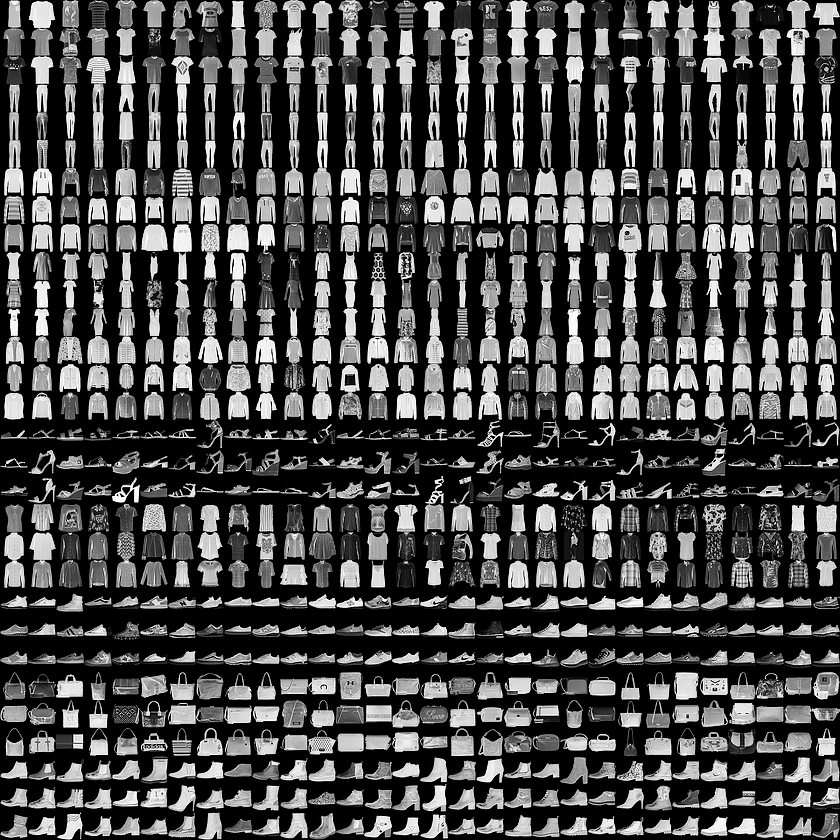
\includegraphics[scale = .4]{resources/fashion_mnist.png}}
\caption{ Visualization of a subset of images from the Fashion MNIST dataset that is trained upon } 
\end{figure}

The Fashion MNIST dataset consists of a 

% Things to address:
%   - Data Preprocessing
% 

\section{Fashion MNIST Results}

\begin{figure}[htbp]
\centering{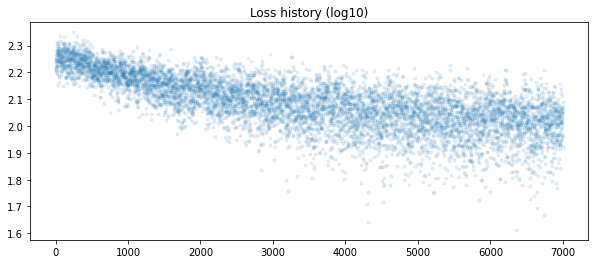
\includegraphics[scale = .4]{resources/test_losspng.png}}
\caption{Three dimensional box plot of the mean hamming distance between the adjusted probabilities on an }
\end{figure}


\begin{figure}[htbp]
\centering{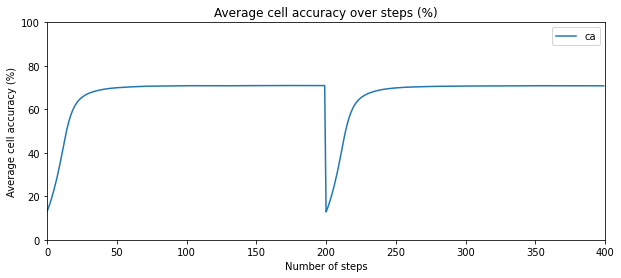
\includegraphics[scale = .4]{resources/test_accuracy.png}}
\caption{Three dimensional box plot of the mean hamming distance between the adjusted probabilities on an }
\end{figure}

\begin{figure}[htbp]
\centering{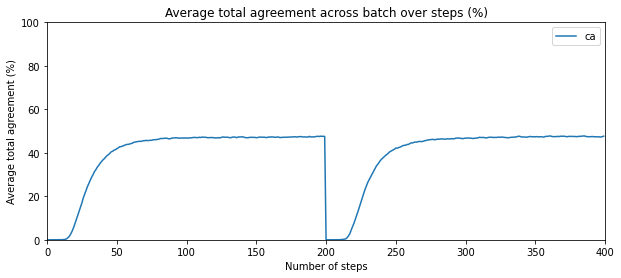
\includegraphics[scale = .4]{resources/test_agreement.png}}
\caption{Three dimensional box plot of the mean hamming distance between the adjusted probabilities on an }
\end{figure}

\subsection{Emulating Germinal Center Capabilities with DEAP}



\section{Discussion}

\subsubsection{Conclusions}


\begin{thebibliography}{00}

\bibitem{self-classify} Randazzo, et al., "Self-classifying MNIST Digits", Distill, 2020.

\bibitem{adversarial} Randazzo, et al., "Adversarial Reprogramming of Neural Cellular Automata", Distill, 2021.

\end{thebibliography}

\section*{Contribution Statements}

\subsection{Connor} 

\subsection{Craig} 

\subsection{Michael} 


\end{document}


